% !TEX TS-program = pdflatex
% !TEX encoding = UTF-8 Unicode

% This is a simple template for a LaTeX document using the "article" class.
% See "book", "report", "letter" for other types of document.

\documentclass[11pt]{article} % use larger type; default would be 10pt

\usepackage[utf8]{inputenc} % set input encoding (not needed with XeLaTeX)
\usepackage{float}
%%% Examples of Article customizations
% These packages are optional, depending whether you want the features they provide.
% See the LaTeX Companion or other references for full information.

%%% PAGE DIMENSIONS
\usepackage{geometry} % to change the page dimensions
\geometry{a4paper} % or letterpaper (US) or a5paper or....
% \geometry{margin=2in} % for example, change the margins to 2 inches all round
% \geometry{landscape} % set up the page for landscape
%   read geometry.pdf for detailed page layout information

\usepackage{graphicx} % support the \includegraphics command and options


% \usepackage[parfill]{parskip} % Activate to begin paragraphs with an empty line rather than an indent

%%% PACKAGES
\usepackage{booktabs} % for much better looking tables
\usepackage{array} % for better arrays (eg matrices) in maths
\usepackage{paralist} % very flexible & customisable lists (eg. enumerate/itemize, etc.)
\usepackage{verbatim} % adds environment for commenting out blocks of text & for better verbatim
\usepackage{subfig} % make it possible to include more than one captioned figure/table in a single float
% These packages are all incorporated in the memoir class to one degree or another...
 \usepackage{longtable} % longtable support required by pandoc >1.10
%%% HEADERS & FOOTERS
\usepackage{fancyhdr} % This should be set AFTER setting up the page geometry
\pagestyle{fancy} % options: empty , plain , fancy
\renewcommand{\headrulewidth}{0pt} % customise the layout...
\lhead{}\chead{}\rhead{}
\lfoot{}\cfoot{\thepage}\rfoot{}

%%% SECTION TITLE APPEARANCE
\usepackage{sectsty}
\allsectionsfont{\sffamily\mdseries\upshape} % (See the fntguide.pdf for font help)
% (This matches ConTeXt defaults)

%%% ToC (table of contents) APPEARANCE
\usepackage[nottoc,notlof,notlot]{tocbibind} % Put the bibliography in the ToC
\usepackage[titles,subfigure]{tocloft} % Alter the style of the Table of Contents
\renewcommand{\cftsecfont}{\rmfamily\mdseries\upshape}
\renewcommand{\cftsecpagefont}{\rmfamily\mdseries\upshape} % No bold!
\usepackage[table,xcdraw]{xcolor}

%%% END Article customizations

%%% The "real" document content comes below...

\title{Functional annotation of Rare and Low Frequency variants of Swedish population on putative enhancer regions identified by HiCAP methods}
\author{Sailendra Pradhananga\\
Science for Life Laboratory/School of Biotechnology\\
Royal KTH institute of Technology (KTH), Swden}
\date{} % Activate to display a given date or no date (if empty),
         % otherwise the current date is printed 

\begin{document}
\maketitle


\section*{Abstract}

GWAS have identified most of variants associated to complex disease to non coding variants. The functional impact of these variants are poorly understood. The non-coding variants are studied using Hi-C and its variant methods such as HiCAP which brings genome into close proximity leading to regulating of gene expression. In current study, we have identified common, low frequency and rare variants one of HiCAP data on two replicates of Bicuspid aortic valve (BAV) heart disease. The current analysis shows that Rare variants are enriched in promoter-mediated putative enhancer. Upon further annotation of these regions with non coding functional markers of DNA hypersensitivity, Histone modification and transcription factor binding sites from public data set shows  $23\%$ these enhancers are enriched with at least one of these markers.  Furthermore, GO term analysis on enhancers with all of these markers points to one of regulation of endothelial tube morphogenesis genes as one with high enhancer changes.

\section{Introduction}
Currently genome wide association studies are targeted to common variants that are present in higher frequency in a population, which had lead into hypothesis of common variant common disease hypothesis. However most of common variants identified so far are within the non-coding regions that are difficult to link with disease. On the other end of spectrum, rare variants: less common in population, are less studied due to large sample requirement and higher cost of sequencing. However, recent studies have shown these genetic variants have higher effect on common diseases as well. 

One of such method to study these variant using HiCap (variant of Hi-C ) methods, that identifies promoter-anchored interaction between variants that are thousand of bases apart from each other. Thus providing connectivity information from GWAS variants with potential genes. HiCAP method generates a genome-wide maps of promoter-anchored chromatin interactions with close to single-enhancer resolution. (cite HiCap methods).  Enhancers are the cis acting regulatory elements of non coding genome which are essential for expression genes. Thus, it would be variation within enhancer region could potential have impact on gene regulation thereby influencing complex diseases.

BAV are the most common type of aortic anomaly that are major common cause of heart disease in adults. BAV are heritable traits with high influencing males than females , however genetics is poorly understood with no clear one gene influencing disease, therby speculating effect of different environmental, genetic and epigenetic factor playing the role in disease.

In the current study we have imputed genetic variants from recently published 1000 Swedish population in promoter mediated putative enhancer from HiCAP. The genetic profile of rare and low frequency variants in interaction data from  are from replicates from BAV heart disease patient. We observed overlap of these enhancer with genetic variants to different functional elements from Chipseq atlas for HUVEC cell line which are primary endothelial cell-lines. 



\section{Materials and methods}

\subsection{Data acquisition}
Whole genome sequencing variant file (vcf) was accessed from SweGen \cite{swegen}  frequency data (https://swegen-exac.nbis.se downloads) of v2. As reported these dataset includes the highest quality genetic map of Swedish population. From the resulting vcf file, the SNP data set was filtered using a vcftools \cite{danecek2011variaDNAsent} in order to separate  snp and indel. Additionally, the variants tagged as "PASS" from GATK \cite{gatk2} was further processed . Further the dark listed genome region \cite{li2014toward} was removed from subsequent analysis.

Additionally , for functional annotation of enhancer regions chipseq atlas \cite{Ohta} data  for DNA hypersensitivity experiments (DNAse HS), H3Kme1  and H327Ac , and transcription factor experiments for HUVEC dataset was accessed. The threshold for experiments was set up at 100 and all the peak files were downloaded.  The DNAse sites have lost their condensed chromatin and are exposed for expression. H3Kme1 and H327Ac are the active markers of  putative enhancers and transcription factor are protein complexes that bind to genome for gene expression. These non coding DNA elements  are putatively functionality markers of potential enhancers. 


\subsection{Definition of Rare and low frequency variant in the population}


The variants from the Swedish population was classified into three separate categories i.e Rare, Low frequncy and common based on the allele frequency  in the population The variant classification were on the frequency such that variant with MAF\textgreater{}0.05 were classified as "Common", Low frequency with 0.05 \textless{} MAF \textless{} 0.01, Rare variants \textless{} 0.01. However in the rare frequency variants were have removed that private variants that were present within one individual either in homozygous or heterozygous condition


\subsection{HI-CAP interaction dataset}

HiCAP experiments on two replicates from BAV patients were performed. The data were preprocessed with each Promoter\-Enhancer  $(P\-E)$ interaction having at greater than three supporting pairs of p-value $< 0.001$ as set in earlier experiments. The final output of the $P\-E$ interaction data consists of information of Promoter in genome, corresponding genes, enhancer position in genome and supporting pair information for each interaction in  two replicates. 

Following the interaction dataset, I developed customized python script $VCFmanipulation.py$  which takes the interaction file and annotates and subsets the enhancer and promoter regions into the rare, low frequency and common regions. Furthermore, I also wrote customized python script $genome_tf.py$ further annotates the DNA elements in these regions.


\subsection {GO term enrichment status of P\_E interaction mediated genes}

GO term of biological processes (BP) that were curated from the GO database were down from QuickGo \cite{quickgo} . Additionally while downloading  the  BP date we considered only the terms that were fulfilled the criteria of manual experiment evidence given in the QuickGO database. We used this criteria in order to limit or gene ontologies analysis to relatively functional genes which have the experimental validation. A customized python $Gene\_ontology.py$ was made in for the following analysis as well.

\section{Results}

\subsection{Rare variants are enriched in putative Promoter - Enhancer Interaction}
There was 35million variants that were tagged as "Pass" all 1000 Swedish genome population. From that, we have identified around 30.2 million SNPs and 4.4 million indels in in the population that are tagged as "Pass" from GATK filter.

We used the customized script *Vcfmaniouation* to overlap the passed SNPs with the enhancer regions. The preprocessed promoter-enhancer list was contained 33,323 unique enhancers regions in Bicuspid aortic valve (BAV cells. The data contains of promoter regions and corresponding enhancer regions of 2 replicates from BAV cell. We found on average of 20.38 and 13.93 interaction enhancers change in replicate1 and replicate2 respectively. As shown in figure 1, we identified  distribution of different enhancer length. 
  
\begin{longtable}[]{@{}lcr@{}}
\toprule
 Enhancer\_length & Counts
type\tabularnewline
\midrule
\endhead
$< 50$kb   & 82591\tabularnewline
$50-500$kb   & 20700\tabularnewline
$500$kb $-1$Mb &  3334\tabularnewline
 $> 1$MB & 1030\tabularnewline
\bottomrule
\end{longtable}

\begin{figure}[H]
\begin{center}
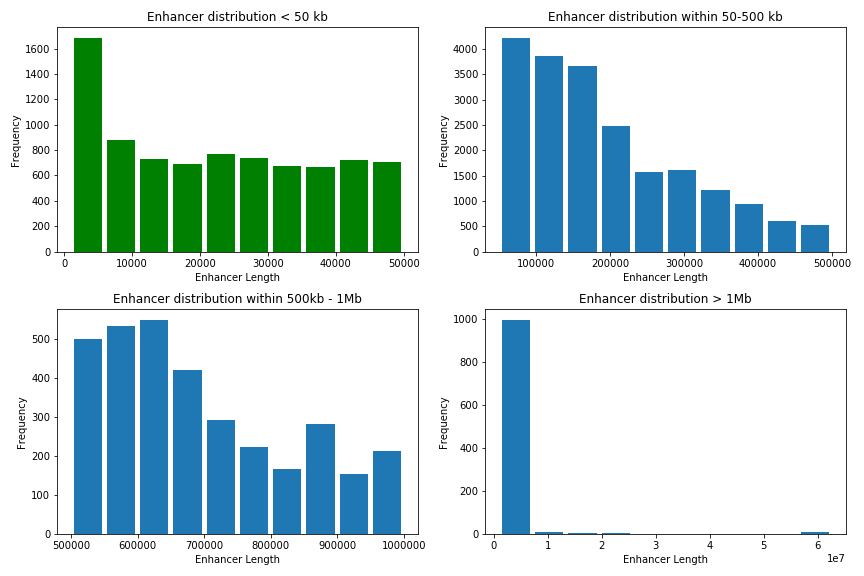
\includegraphics[width=\textwidth]{length_distribution}

\caption{Mapping status in both platform. {\bf A} Raw reads counts in WES and WGS. {\bf B}  Duplicated reads in each sample in WES and WGS}
 \label{duplcated}
\end{center}
\end{figure}

This length distribution depicts that most of our putative enhancers are within the range of 50-1Mb base pairs which is in par with the Hi-C methods

We identified  22,055, 14403 and 22,144 putative enhancer regions in our interaction dataset with common, low-frequency and rare variants. Furthermore, we identified in total 56,891 common , 24,049 low-frequency and  47,281 rare variants enriched in these enhancer regions as shown in table 2. Interestinly, our enhancer regions have been enriched with rare variants from the population.

\begin{longtable}[]{@{}lcr@{}}
\toprule
Variant class & Enhancer with variants & Total variants
type\tabularnewline
\midrule
\endhead
Common & 22055 & 56891\tabularnewline
Low Frequency & 14403 & 24049\tabularnewline
Rare & 22144 & 47281\tabularnewline
\bottomrule
\end{longtable}


\subsection{Status of non coding functional DNA elements of variants embedded enhancer regions}

We observed the following non coding functional elements in each of three separated annotated dataset table 2 and figure 2

\begin{figure}[H]
\centering
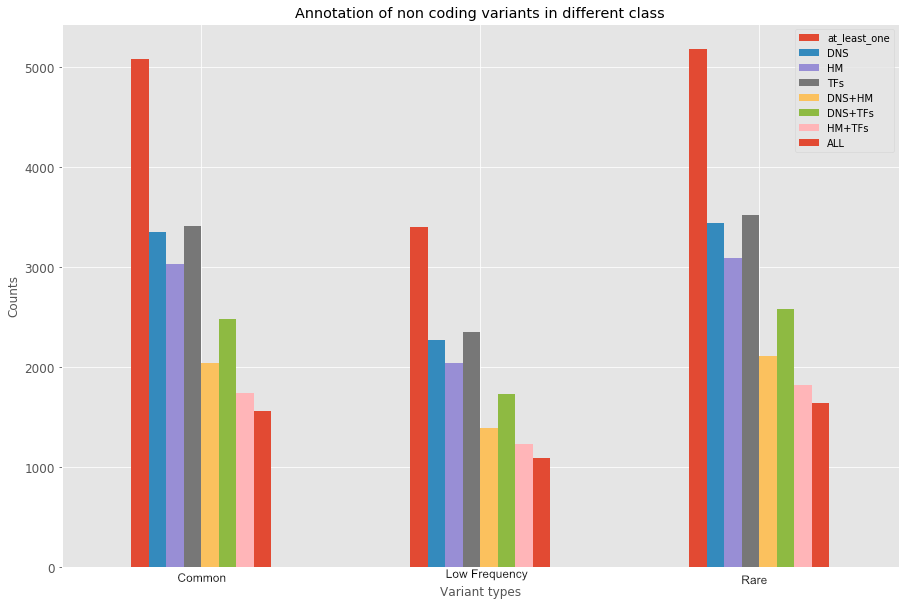
\includegraphics[width=\textwidth]{../Enhancer_elements.png}
\caption{figures 3}
\end{figure}

\begin{table}[H]
\centering
\label{my-label}
\begin{tabular}{@{}lllllllll@{}}
\toprule
\rowcolor[HTML]{BBDAFF} 
\multicolumn{1}{c}{\cellcolor[HTML]{BBDAFF}{\color[HTML]{333333} class}} & {\color[HTML]{333333} at\_least\_one} & {\color[HTML]{333333} DNS} & {\color[HTML]{333333} HM} & {\color[HTML]{333333} TFs} & {\color[HTML]{333333} DNS+HM} & {\color[HTML]{333333} DNS+TFs} & {\color[HTML]{333333} HM+TFs} & {\color[HTML]{333333} ALL} \\ \midrule
\cellcolor[HTML]{FFFFFF}Common & 5087 & 3350 & 3029 & 3416 & 2042 & 2487 & 1744 & 1565 \\
\cellcolor[HTML]{FFFFFF}Low Frequency & 3407 & 2276 & 2038 & 2356 & 1393 & 1736 & 1229 & 1095 \\
\cellcolor[HTML]{FFFFFF}Rare & 5178 & 3440 & 3097 & 3524 & 2114 & 2587 & 1820 & 1638 \\ \bottomrule
\end{tabular}
\end{table}

From the above chart, it can been said that we have at least one of functional markers in about (5087/22055) 23\% of putative enhancer in all classes of variants. However, it has to be considered that we took into consideration one of cell line and these are the markers specific to cell type. Most interesting , we still find at least 1000 putatively, functional enhancers in all classes in all. It would be interesting to observe these functional enhancer regions and dig into Rare and Low frequency variants in these region.Furthermore, these are result only from overlapping with one dataset. This data has to be randomized and overlapped so as to find the putative p-values to our non coding functional elements.

\subsection{GO term enrichment status of P\_E interaction mediated genes}


We found 2 enriched GO Terms at descending order of enhancer per gene and number of enhancer mediated\_promoter gene \textgreater{} 2 in rare and Low frequency variants i.e GO:1902894 regulation of pri-miRNA
transcription from RNA polymerase II promoter GO:1901509 regulation of endothelial tube morphogenesis.

\section{Discussion}

In the current report we have presented the status of genetic variants identified from Swedish population in the putative enhancer genomic regions mediated by promoter-enhancer mediated interaction (PEI). These PEIs were called using HiCAP experiments in replicates of BAV heart disease patient.  Our analysis depicts that rare variants are enriched within our enhancer regions which was as expected since these rare variants also contains the variants which might be presented in one individuals as we haven't corrected for homogenous individuals. However we still find variants which are presented at least greater than five allele counts . 

Based on the definition rare, low frequency and common variants, we annotated our enhancer with active enhancers marks. We used publicly available HUVEC dataset for chipseq atlas on DNAse Hypersensitivity. These regions provided the accessibility of genome for  further processing . In the same enhancers regions we annotated with active enhancers histone marks (H327ac and H3Kme1) and transcription factor binding sites. The formation of complex between TFs, enhancers and promoter have been already reported as fundamental mechanism for regulation of trancription \cite{mora2015loop}.  At the current analysis, we find more than enhancer regions which have been all of these functional marks. This is still a lower number and tested within one type of cellline. Based on the this result, we are unable to claim whether these are functional or not. Furthermore, from this primary analysis, we have to calculate enrichment status based on random distance mediated enhancer.

GO-Term analysis have represented regulation of endothelial tube morphogenesis as one of GO with high enhancer activity in rare and low frequency class of variants. Endothelial progenitor cells have been associated as biomarker of cardiovascular disease \cite{grisar2011endothelial}.  There has been elucidation of endothelial cells in relation to inflammation in vascular disorders. Thus, the genes associated i.e FOXP1 and FGF1 and their corresponding enhancer could have functional implication in understanding disease prognosis. However these genes and GO term analysis needs further processing.


\section{Conclusion}

We have used currently available large scale genetic frequency data in homogenous Swedish population to identify the promoter mediated enhancer enriched with rare variants. Upon further annotation of these enhancer with functional markers lead to identification of interesting GO-terms. Although HICAP based enhancer analysis is currently fully mature, we believe that preliminary results points that rare variants could potentially driving the complex phenotypes such as BAV heart disease.

\newpage


\bibliographystyle{unsrt}
\bibliography{report_17th_Oct}



















\end{document}
